\chapter{Scaling laws}\label{ch:scalinglaws}
One of the goals of this work is to search, reveal, study and use universal laws in bulk gene expression data~\nocite{altmann2016statistical}.
As in chapter~\ref{ch:structure} approaches from different field of science are considered at this point.

In can be interesting to study the behaviour of the gene expression across samples.

\section{Scaling}
\draft{gene expression across samples? gamma?}

Given a matrix of components and realisations as~\ref{fig:componetstable} with expression entries $n_{i j}$ it is possible to estimate the mean of a row $m_i=\avg{n_{i
 j}}_j$ and its variance $\var{i}=\avg{n_{i j}^2}_j - \avg{n_{i j}}^2_j$.

\paragraph{Variance versus mean}\mbox{}\\
First of all, it could be interesting to study the variance of expression $\var{\mathrm{counts}}$ versus its average $\avg{\mathrm{counts}}$ across tissues.
%%all genes
\begin{figure}[htb!]
    \centering
    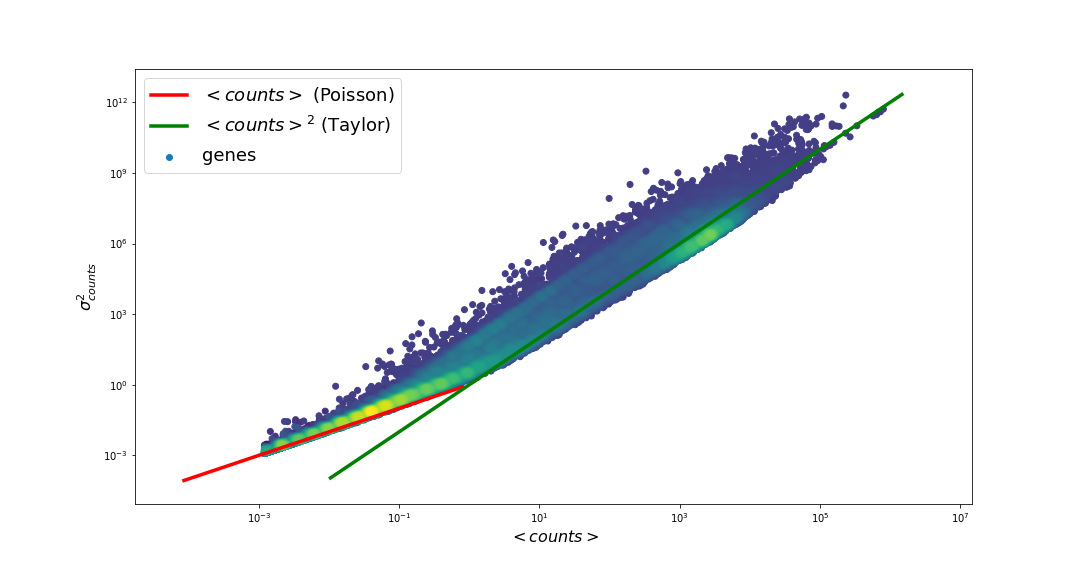
\includegraphics[width=0.9\linewidth]{pictures/scalinglaws/gtex/allgenes/varmean_loglog.png}
    \caption{Variance versus average. In \textcolor{pythonred}{red} the Poisson-like scaling, in \textcolor{pythongreen}{green} the Taylor-like scaling. All genes are considered.}
    \label{fig:scalinglaws/gtex/allgenes/varmean_loglog_density}
\end{figure}
In figure~\ref{fig:scalinglaws/gtex/allgenes/varmean_loglog_density} the scatter plot of variance versus mean reveals some interesting facts.
First of all, it is evident that data have a double scaling behaviour: when the mean is small ($\lesssim 1$) data scale a Poisson-like ($\var{\mathrm{counts}} \sim \avg{\mathrm{counts}}$), at higher means data present instead a quadratic scaling ($\var{\mathrm{counts}} \sim \avg{\mathrm{counts}}^2$) known in ecology as Taylor's law~\cite{Eisler2008}. This means that at low averages data's behaviour is due to the sampling process; on the contrary, Taylor's law reveals the non-trivial distribution across samples of the gene expression.

Another interesting fact is that looking at the density of points (colours in figure~\ref{fig:scalinglaws/gtex/allgenes/varmean_loglog_density}) two clouds of points emerge: one at low averages and one at high averages. These correspond to coding and non-coding genes, remembering section~\ref{sec:universallaws} these two kind of genes have different behaviours: protein-coding genes are highly expressed in the majority of the samples, non-coding ones are less expressed (and so less sampled) in a few samples. 

\paragraph{Coefficient of Variation}\mbox{}\\
A similar analysis, common in literature, is the analysis of the coefficient of variation squared $CV^2=\frac{\var{\mathrm{counts}}}{\avg{\mathrm{counts}}^2}$ represented in figure~\ref{fig:scalinglaws/gtex/allgenes/cvmean_loglog}.
\begin{figure}[htb!]
    \centering
    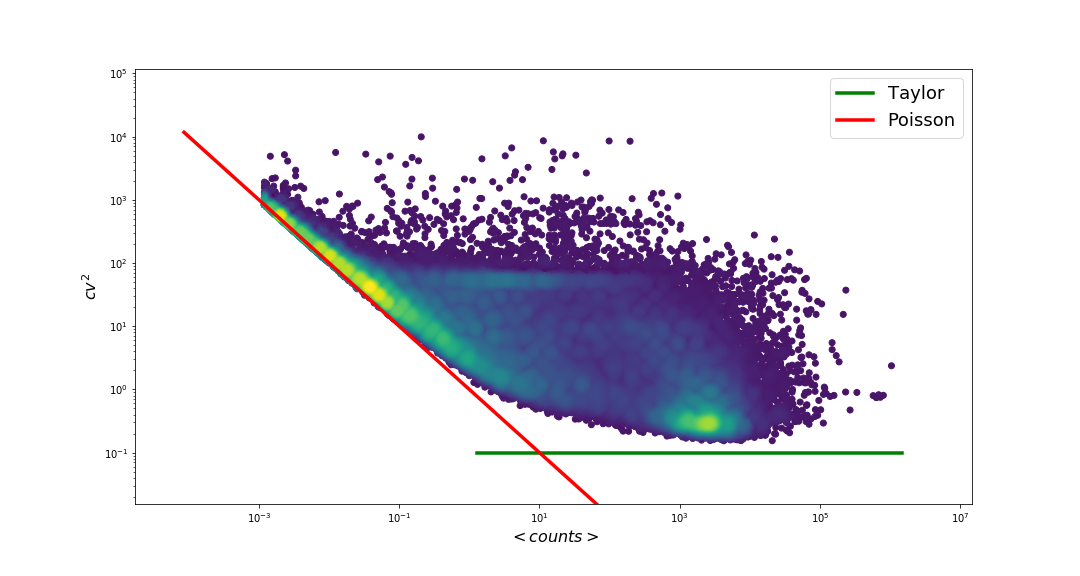
\includegraphics[width=0.95\linewidth]{pictures/scalinglaws/gtex/allgenes/cvmean_loglog.png}
    \caption{Coefficient of variation squared versus average. In \textcolor{pythonred}{red} the Poisson-like scaling, in \textcolor{pythongreen}{green} the Taylor-like scaling. All genes are considered.}
    \label{fig:scalinglaws/gtex/allgenes/cvmean_loglog}
\end{figure}
The behaviour is complementary to the one discussed above; a double scaling, quite common in the literature looking at single-cell RNA sequencing data~\cite{Islam2013}, is present. Even looking at $CV^2$ it is evident the presence of the protein-coding and non-coding clouds of points. The non-coding genes have a Poisson-like scaling, $\var{\mathrm{counts}} \sim \avg{\mathrm{counts}}$ so $CV^2=\frac{\var{\mathrm{counts}}}{\avg{\mathrm{counts}}^2}\sim\frac{1}{\avg{\mathrm{counts}}}$, otherwise the protein-coding genes are on the Taylor-like curve $CV^2=\frac{\var{\mathrm{counts}}}{\avg{\mathrm{counts}}^2}\sim \text{constant}$.

\paragraph{Protein-coding genes} can be isolated and considered on their own. The same analysis confirms that the cloud of points on the Taylor-like scaling is made by protein-coding genes.
\begin{figure}[htb!]
    \centering
    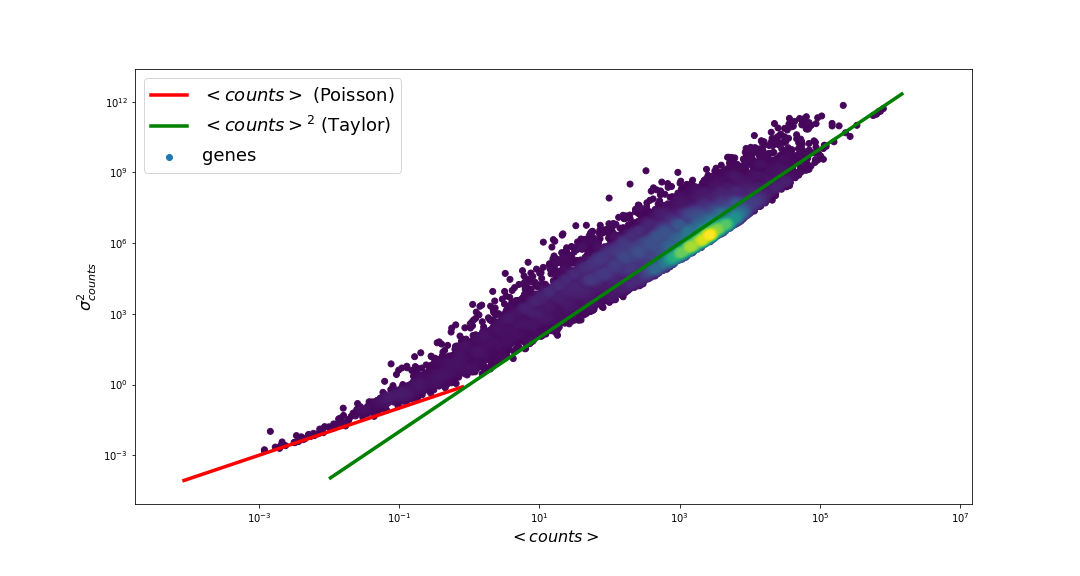
\includegraphics[width=0.95\linewidth]{pictures/scalinglaws/gtex/varmean_loglog_density.png}
    \caption{Variance versus average. In \textcolor{pythonred}{red} the Poisson-like scaling, in \textcolor{pythongreen}{green} the Taylor-like scaling. Only protein-coding genes are considered.}
    \label{fig:scalinglaws/gtex/varmean_loglog_density}
\end{figure}

Following the sampling model of~\cite{Mazzolini2018} summed up in section~\ref{sec:nullmodel} the averages and variances can be estimated on null matrices. In figure~\ref{fig:scalinglaws/gtex/varmean_3sigma} the comparison between real genes and sampling data. The sampling has got a double scaling as well; this is quite interesting, it means that the global scaling is due to the Zipf distribution and the sizes' distribution themselves, they are, by definition, identical in the data and in sampling.
Moreover, the sampling points draw a lower bound of the data, this encodes the information that the data are more variable (have higher variance) than just sampling, so there must be some biological information hidden that causes this over-variable behaviour.
\begin{figure}[H]
    \centering
    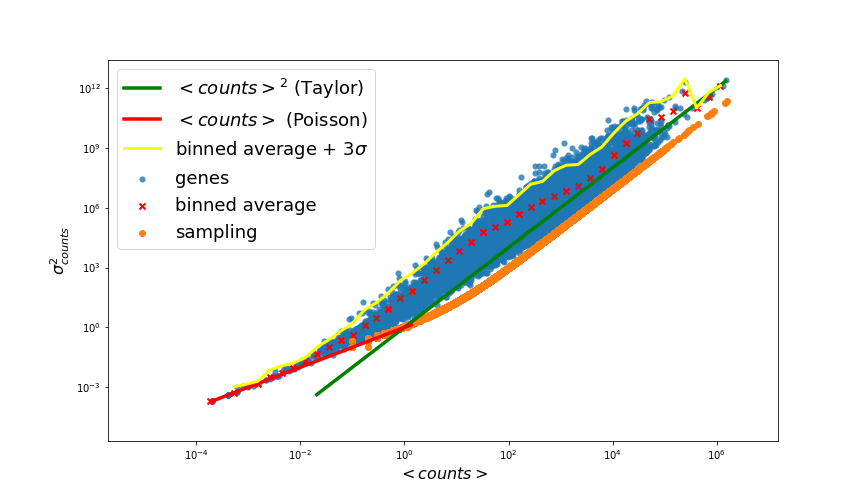
\includegraphics[width=0.8\linewidth]{pictures/scalinglaws/gtex/varmean_3sigma.png}
    \caption{Variance versus average. In \textcolor{pythonred}{red} the Poisson-like scaling, in \textcolor{pythongreen}{green} the Taylor-like scaling. In \textcolor{pythonorange}{orange} the sampling components. Only protein-coding genes are considered.}
    \label{fig:scalinglaws/gtex/varmean_3sigma}
\end{figure}

Again it is possible to analyse the $CV^2$, this time considering only protein-coding genes. Figure~\ref{fig:scalinglaws/gtex/allgenes/cvmean_loglog} confirms that the cloud of points near the Taylor-like scaling is made of protein-coding genes and a double scaling is seen once again.
\begin{figure}[htb!]
    \centering
    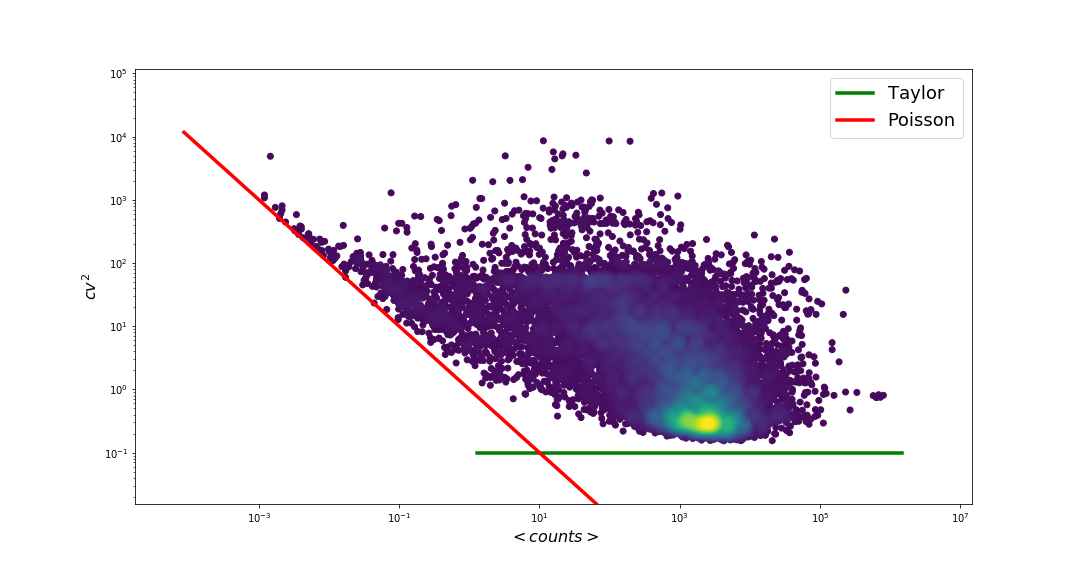
\includegraphics[width=0.9\linewidth]{pictures/scalinglaws/gtex/cvmean_loglog_density.png}
    \caption{Coefficient of variation squared versus average. In \textcolor{pythonred}{red} the Poisson-like scaling, in \textcolor{pythongreen}{green} the Taylor-like scaling. Only protein coding genes are considered.}
    \label{fig:scalinglaws/gtex/cvmean_loglog}
\end{figure}

In figure~\ref{fig:scalinglaws/gtex/cvmean_loglog_sampling} the same plot compared to the sampling data. The double scaling is evident also for the sampling points. Note that $CV^2$ has got a lower bound at $0$ which corresponds to the less variable case: all expressions are identical in all samples ($\var{\mathrm{counts}}=0$). There is an upper bound at $R-1$, with $R$ the number of realizations, that corresponds to the most variable case: a component expresses in only one realization and is $0$ elsewhere.
\begin{figure}[htb!]
    \centering
    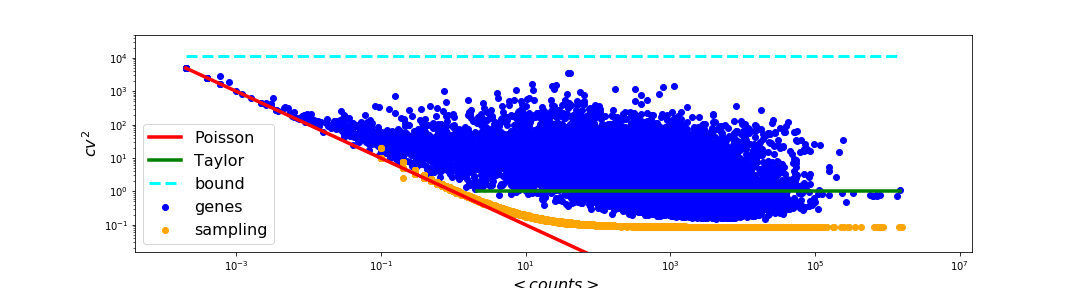
\includegraphics[width=0.9\linewidth]{pictures/scalinglaws/gtex/cvmean_loglog_sampling.png}
    \caption{Coefficient of variation squared versus average. In \textcolor{pythonred}{red} the Poisson-like scaling, in \textcolor{pythongreen}{green} the Taylor-like scaling. In \textcolor{pythonorange}{orange} the sampling components.}
    \label{fig:scalinglaws/gtex/cvmean_loglog_sampling}
\end{figure}

Finally, the data have a double scaling when looking at their global variance across realizations, a Poisson-like scaling in the region where the sampling experimental process is more important and a Taylor-like scaling where the complexity of the data emerges.
Non-coding genes have got low expression and are rare; protein-coding genes, otherwise, express a lot and everywhere and carry more information; this behaviour results in a double scaling. All genes are more variable than a sampling null model and this is the evidence that something interesting is hidden behind the data.


\paragraph{$<FPKM>$ normalisation}
One can be interested in finding genes that are expressed often, and what is the
average expression of them.
To manage this it is plotted the average expression $<FPKM>$ versus the number
of samples in which that gene is expressed that is, considering the thresholds~\ref{sec:threshold},
$\Sigma_j\theta (FPKM_{ij}-0,1)\theta (10^5-FPKM_{ij})$

\subsection{Average versus occurrence}
Another interesting analysis can be the relation between the occurrence and the average. In figure~\ref{fig:scalelaws/gtex/meanDiff_binned_sampling} it is shown the re
sult, it is clear that there is a relation between occurrence and average, genes that express in more realisations (higher occurrence and right in the figure) have an
higher average. Moreover doesn't exist genes that have high expression in few realisations; genes that are rare are also difficult to find so have a small average. Not
e that the average has got a bound due to the fact that counts are integer numbers, so if, for example, one gene express in $n$ of the $R$ samples, it has occurrence $
O_i=\frac{n}{R}$ and its average is at least $\avg{\mathrm{counts}}=\frac{1*n}{R}$
\begin{figure}[htb!]
    \centering
    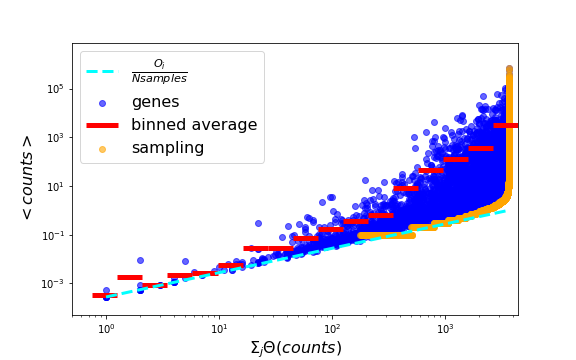
\includegraphics[width=0.9\linewidth]{pictures/scalelaws/gtex/meanDiff_binned_sampling.png}
    \caption{Relation between the occurrence of a gene and its average across realisations}
    \label{fig:scalelaws/gtex/meanDiff_binned_sampling}
\end{figure}

\subsection{Tissue differentiation}
Per gene type scaling
